\documentclass[10pt,journal,cspaper,compsoc]{IEEEtran}
\usepackage[]{lipsum}
\usepackage{cite}
\usepackage{amsmath,amssymb}
\usepackage{algorithm}
\usepackage{algorithmic}
\usepackage{multirow}

\usepackage[aboveskip=8pt]{caption}

\usepackage[dvips]{graphicx}
\DeclareGraphicsExtensions{.pdf}
\usepackage[american]{babel}

\usepackage{tabularx}


\usepackage{url}
\usepackage{cvpr}
\usepackage{multicol}

\usepackage{stfloats}
\usepackage{fixltx2e}
\usepackage{subfig}
\usepackage[bookmarks=false,colorlinks=true,linkcolor=black,citecolor=black,filecolor=black,urlcolor=black]{hyperref}

\newcommand{\cb}[1]{\textbf{#1}}
\newcommand{\ct}[1]{\fontsize{7pt}{1pt}\selectfont{#1}}
\newcommand{\tn}[1]{\footnotesize{#1}}
\newcolumntype{x}{>\small c}


\def\cls{\mathit{cls}}
\def\reg{\mathit{reg}}

%\renewcommand{\floatpagefraction}{0.1}
%\renewcommand{\bottomfraction}{0.1}
%\renewcommand{\topfraction}{1}
%\renewcommand{\textfraction}{0.0}
\renewcommand{\dbltopfraction}{1.0}
\renewcommand{\dblfloatpagefraction}{0.0}

\newcommand{\tabincell}[2]{\begin{tabular}{@{}#1@{}}#2\end{tabular}}

\title{Mine-RCNN}

\begin{document}


    \author{Loi~Dario (1940849),
        Marincione~Davide (1927757),
        Barda~Benjamin (1805213)% <-this % stops a space
    }
%\IEEEcompsocitemizethanks{
%\IEEEcompsocthanksitem S. Ren is with University of Science and Technology of China, Hefei, China. This work was done when S. Ren was an intern at Microsoft Research. Email: sqren@mail.ustc.edu.cn
%\IEEEcompsocthanksitem K.~He and J.~Sun are with Visual Computing Group, Microsoft Research. E-mail: \{kahe,jiansun\}@microsoft.com
%\IEEEcompsocthanksitem R.~Girshick is with Facebook AI Research. The majority of this work was done when R. Girshick was with Microsoft Research. E-mail: rbg@fb.com}
%}

\IEEEcompsoctitleabstractindextext{%
\begin{abstract}
    Real time object detection has recently been made possible due to steady state-of-the-art advancements in the field \cite{arxiv:FastRCNN,arxiv:FasterRCNN}, these methods propose the use of a Region Proposal Network to 
    identify Regions of Interest (RoIs) in the image and correctly classify them, we aim to reproduce the architecture proposed by \cite{arxiv:FasterRCNN} applied to a novel environment, that of the
    popular sandbox Minecraft, both for the ease-of-collection of the required data and for a number of graphical properties possesed by the game that make such a complex problem more approachable in terms 
    of computational resources, moreover, due to the novelty of the environment, we also train the entirety of the network from the ground up, having no pre-trained backbone at our disposal.
\end{abstract}

%State-of-the-art object detection networks depend on region proposal algorithms to hypothesize object locations. Advances like SPPnet and Fast R-CNN have reduced the running time of these detection networks, exposing region proposal computation as a bottleneck. In this work, we introduce a Region Proposal Network (RPN) that shares full-image convolutional features with the detection network, thus enabling nearly cost-free region proposals. An RPN is a fully convolutional network that simultaneously predicts object bounds and objectness scores at each position. The RPN is trained end-to-end to generate high-quality region proposals, which are used by Fast R-CNN for detection. We further merge RPN and Fast R-CNN into a single network by sharing their convolutional features---using the recently popular terminology of neural networks with 'attention' mechanisms, the RPN component tells the unified network where to look. For the very deep VGG-16 model, our detection system has a frame rate of 5fps (including all steps) on a GPU, while achieving state-of-the-art object detection accuracy on PASCAL VOC 2007, 2012, and MS COCO datasets with only 300 proposals per image. In ILSVRC and COCO 2015 competitions, Faster R-CNN and RPN are the foundations of the 1st-place winning entries in several tracks. Code has been made publicly available.

% Note that keywords are not normally used for peer review papers.
\begin{IEEEkeywords}
 Object Detection, Convolutional Neural Network, Sandbox, Region Proposal, Real Time Detection
\end{IEEEkeywords}}

\maketitle
\IEEEpeerreviewmaketitle
    
\begin{figure*}[tb]
    
    \centering
    \subfloat[Our Backbone]{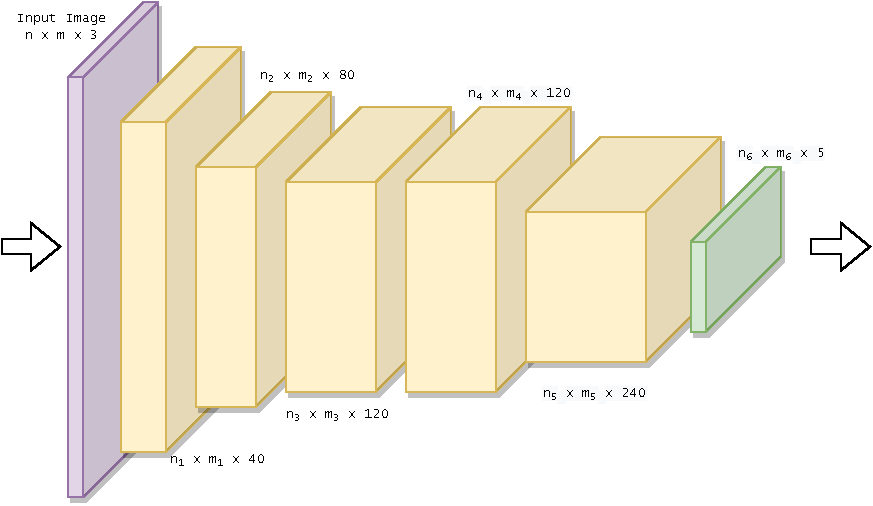
\includegraphics[width=0.45\textwidth]{images/backbone.pdf}} \hfill
    \subfloat[Our Network]{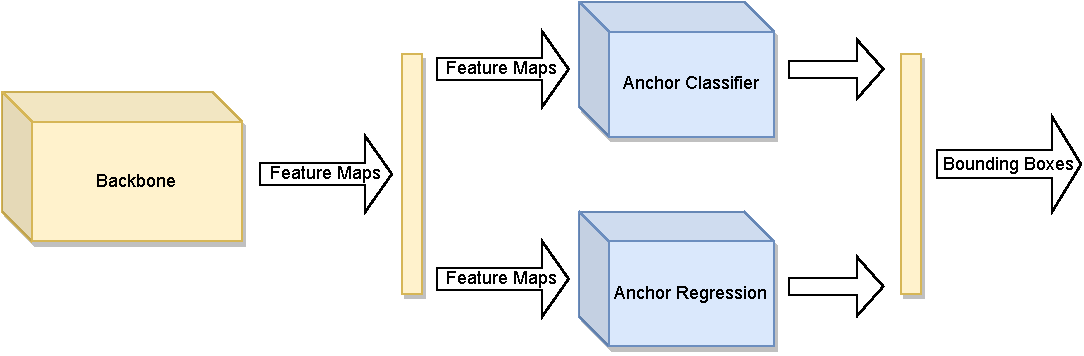
\includegraphics[width=0.45\textwidth]{images/network.pdf}}
    \caption{Our FCNN backbone (a) employes a series of convolutions to obtain a feature map to pass to 
    the rest of the network as displayed in (b), the feature maps from our Backbone are first pre-processed
    by a sliding-window approach that spreads our anchors over the image, this is then passed to a twin neural
    network, one part of the network performs classification, determining if each bounding box is containing an
    object or not, the other part performs regression on our bounding box in order to make it better fit an eventual
    target object.}
    \label{fig:network}
\end{figure*}


\begin{figure}[tb]
    \centering
    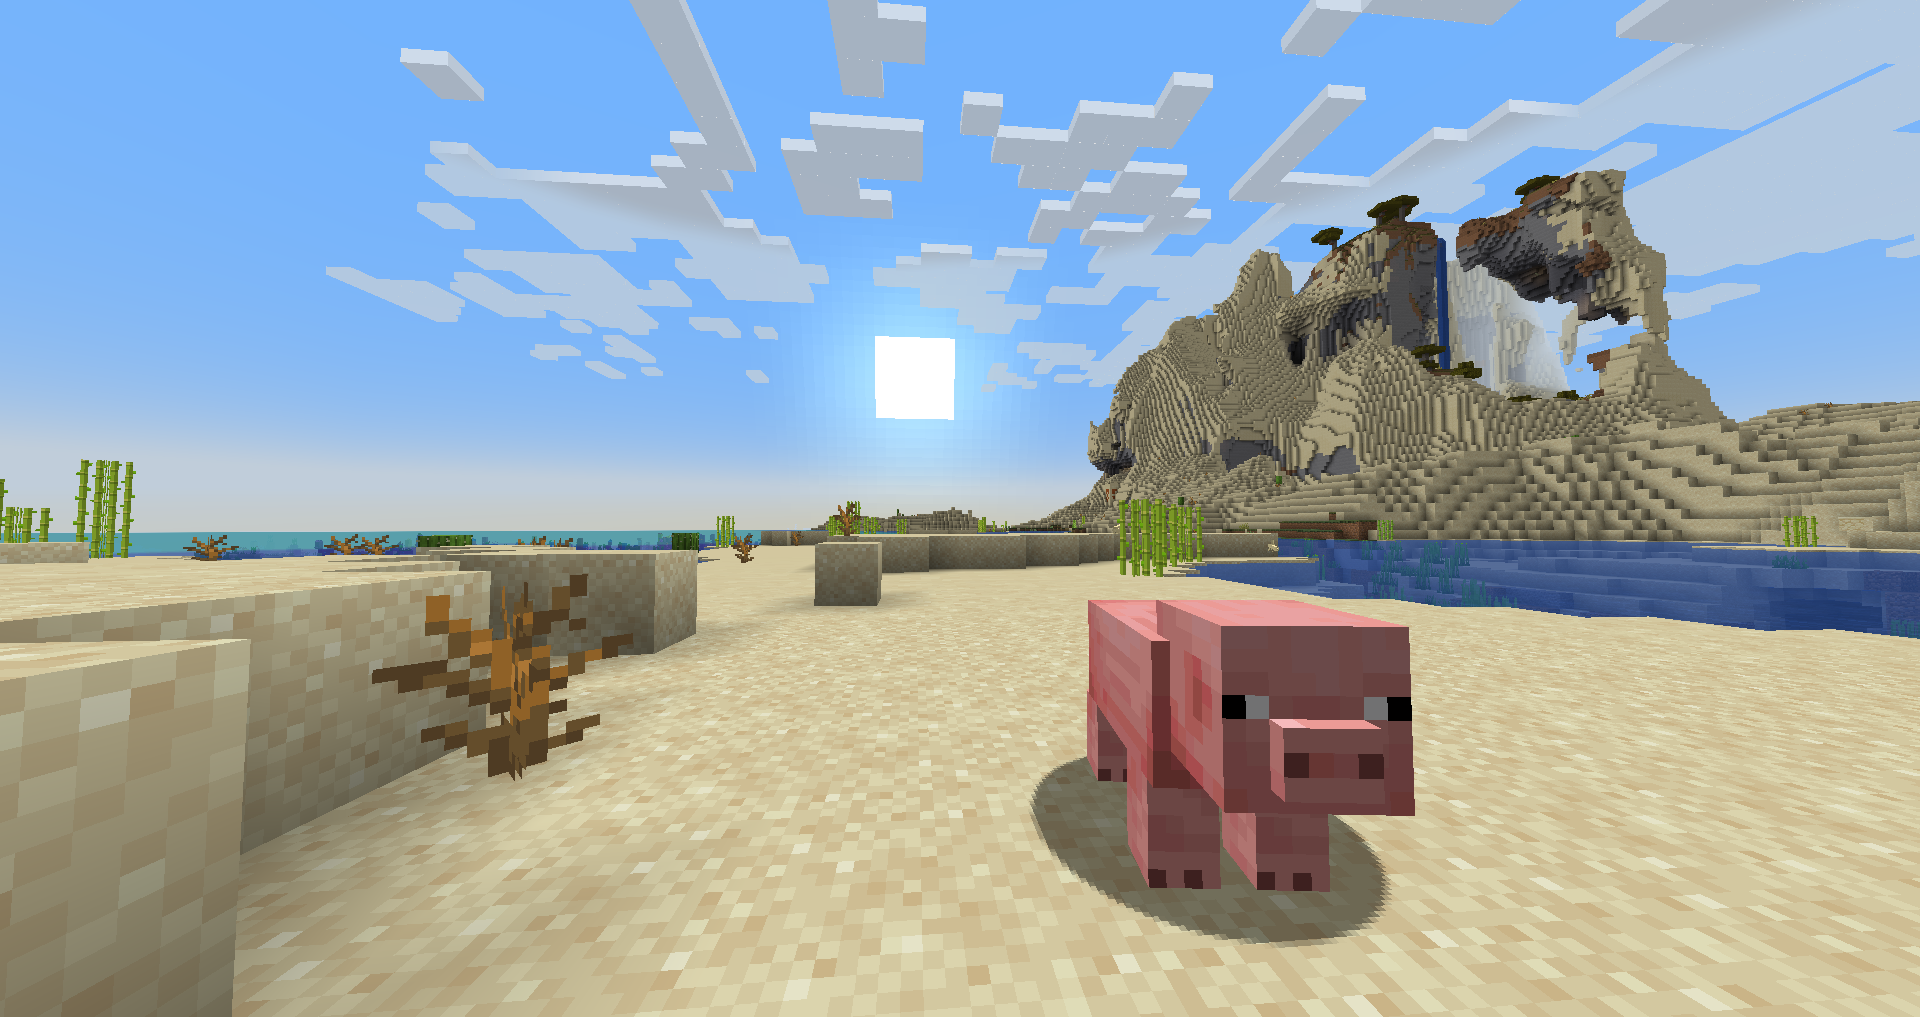
\includegraphics[width=0.44\textwidth]{images/pig.png}
    \caption{A Screenshot of the world of Minecraft, note the simplistic graphics and the absence of Bloom (except the illusion thereof provided by the 
    skybox) even though we are staring directly at the sun, note also the presence of a \emph{pig}, one of the entities that we are going to detect 
    in our model.}
    \label{fig:piggy}
\end{figure}

    \section{Introduction}
    Traditional visual recognition algorithms employ the use of algorithms such as SIFT 
    or SURF\cite{Lowe:SIFT,Bay:SURF}, to extract a feature descriptor from key points 
    in the image, a set of sample images is therefore processed in order to obtain descriptors 
    for each class, inference is then performed by extracting the descriptor from the input image 
    and then comparing it with our samples, using a distance criterion to select the closest class.

    While these traditional methods are mostly invariant to scale and translations, issues such as 
    variability in the brightness or rotation of the target object are problematic, moreover, the 
    computational cost of extracting features is prohibitively high, effectively preventing the possibility
    of deploying the model in a real-time context.

    \paragraph*{Our Approach}
    One way to reduce the cost in performance while gaining a higher expressive capacity for our model is to employ
    modern Deep Learning techniques to build our detector, our aim is therefore to 
    design a scaled-back version of \cite{arxiv:FasterRCNN}, stopping ourselves at the classification stage,
    the reason for this will be further clarified in the rest of the paper, our architecture\footnote{see 
    Figure \ref{fig:network} for a diagram
    of our architecture} is composed of a FCNN\cite{Chen:FCNN,Simonyan:VCC16} Backbone, this is to keep the number 
    of parameters as low as possible as well as allow the initial layer of our architecture to be applicable to images 
    of any resolution, our Convolutional Backbone must be trained from the ground up in the task of simply classifying 
    the classes that we intend to detect, the classifying layer is then removed from the model and we're then
    left with its feature map output which we then pre-process by \emph{splashing} anchors through a sliding window 
    approach.

        

    After this, both feature maps and anchors are then passed to our region proposal layers, which in turn is composed 
    of a twin ensemble of Neural Networks that perform Regression and Classification on the bounding boxes, the outcome is a set of 
    \emph{positive} and \emph{negative} bounding boxes, the boxes that are classified as positive 
    go through NMS\cite{Neubeck:NMS} using Intersection over Union (IoU) \cite{Rezatofighi:IoU} as a metric for suppression
    in order to reduce the amount of individual boxes that classify the same object.

    
    \paragraph*{Our Environment}
    In order to keep our project in the realms of feasibility, especially considering the constraints imposed on our team in the 
    realms of time and processing capabilities of our hardware, we chose to detect objects in a virtual environment, this is because 
    the possibility of having complete control over the environment allows us to artificially create scenarios from which we can gather 
    samples of a large quantity, for this reason, we chose the popular sandbox game Minecraft \cite{Mojang-Minecraft}, other than 
    the advantage of control over the environment, the game is well known for it's simplistic approach to Voxel Graphics, rendering 
    the world as a set of blocks of cubic shape, the game also possesses a simplistic lightning model that simply shifts the brightness
    of blocks' textures when in the vicinity of a light source, thus being void of effects such as bloom, specular components on objects,
    reflections and other complex techniques that introduce sources of unexpected noise or variability in our samples, this, in turn, 
    allows our model to work in a context that, while still posing a significant challenge, is of suitable difficulty to the scope of 
    this project.



    \section{Method}
    \paragraph*{The Dataset}
    We started first by building the dataset. We recorded one-minutes long videos of Minecraft using commercial screen captures softwares. We then loaded those shorts into python, using the OpenCV library, in order to sample one frame per second as we 
    beleived would have given enough time for the next sampled frame to have significative diffrences with respect to the previous ones. We then downsampled the images in order to compress the size of the dataset in order to be able to share it with ease. To further 
    reduce the problem we adopted for the final image a one-to-scale ratio, thus making the image squared. At this time we opted to limit ourselves to only five classes we were aiming to classify: Zombies, Creepers, Pigs, Sheeps, Nothing. 
    The next step was labeling each sampled frames. We developed a simple but effective tool that allowed us to draw boundng boxes(BBox), and assign to each one of them a label corresponding to a class mentioned above. During this process we pruned images that we considered
    unfit to be part of the dataset (e.g. frames inside the game menu or outside of the game). After standardizing the coordinates of BBoxes we saved them into JSONs files. Having our JSONS files ready we group them into a single .dtst file for better integration with the PyTorch
    library, which is the one we decided to use for this project. From the sampling of the images we collected 3920 valid frames. 
    
    \section{Results}
    Given the inexperience, the difficulty of the task and the (inadequate) hardware at hand, we think to have reached positive results, the system shows signs of being able to recognize traits of the mobs we've trained it on, even though sometimes they are just cases of pareidolia. Before giving some manner of statistics over its capabilities we would like to point out an important decision: that of the threshold for deciding whether, given a score, the anchor for which it is related to is actually a positive one or not. To decide this fundamental hyperparameter we resolved in sampling five hundred (500) images from our training dataset and, after letting the system apply non-maximum suppression, recovering the scores for all the remaining anchors and pairing them to their true labels. Once this preprocessing was done we plotted the ROC:

    \begin{figure}[h]
        \centering
        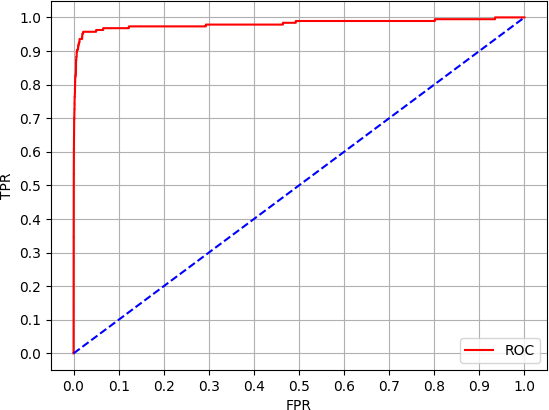
\includegraphics[width=0.44\textwidth]{images/ROC.png}
    \end{figure}

    And a graph, showing the decrease of the \emph{true positive ratio} (TPR) and of the \emph{false positive ratio} (FPR) as the threshold increased, as following:

    \begin{figure}[h]
        \centering
        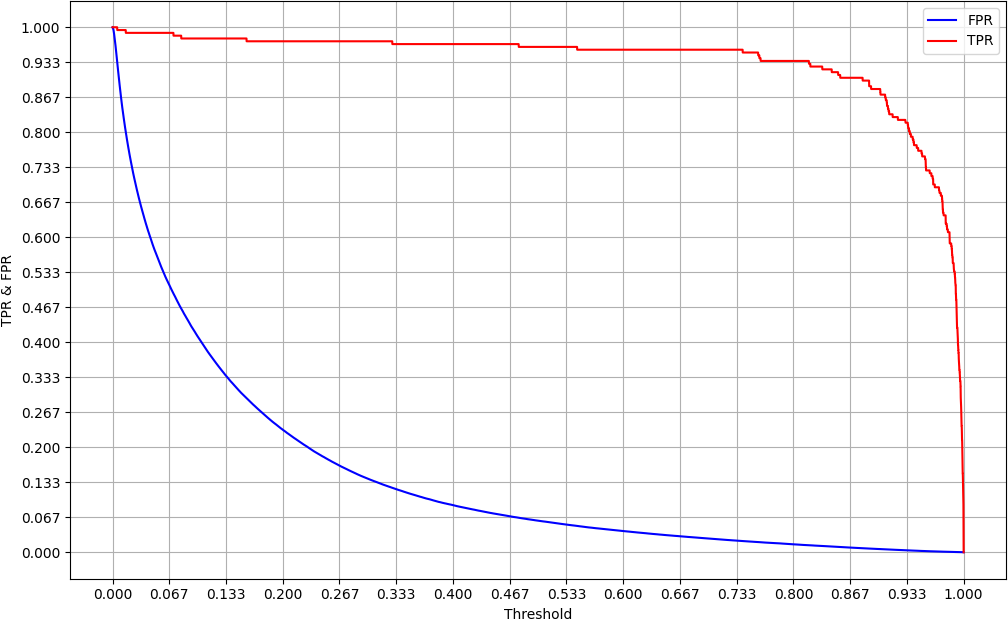
\includegraphics[width=0.44\textwidth]{images/threshold_decision.png}
    \end{figure}

    From both these graphs we notice our network is indeed able to separate positive and negative anchors with very clear-cut definition. Furthermore, we decided that a good compromise between (TPR) and (FPR) could be achieved by choosing a threshold between $0.8$ and $0.9$: since we didn't want to remove positive anchors too much we put ours at $0.81$. We posit that, to avoid false positives as much as possible, $0.9$ should work fine too.

    After this, in our opinion, fundamental decision was made: we resolved to open Pandora's box and create a test set of around 250 images with multiple mobs in the same shot. Unfortunately, as said previously, we didn't develop our network up to classification of the boxes, and thus a full confusion matrix of those is out of the question. At any rate we show the misclassification table for the anchors (after non-maximum-suppression) scored by our network over the whole test set:

    \begin{center}
        \begin{tabular}{r|c c}
            & Pos. label & Neg. label \\
            \hline
            Pos. score & 62 & 3545 \\
            Neg. score & 17 & 127789
        \end{tabular}
    \end{center}

    Telling us that, indeed, our threshold works, since the TPR is $0.78$ and the FPR is $0.03$. We would like to point out that, since the labelling of the anchors is itself hyperparameter driven (given the choice of anchors and that of the IoU thresholds used to label them) and that we think to have chosen a combination of these parameters that biases the labels towards the non-object side and, furthermore, given this label by itself already dominates the distribution: it is only normal for the number of positive labels to be so low in the set. If we look at the actual images with the positive region proposals added, we'll appreciate much more positive-looking (that may not actually be labelled as positive) proposals than the anchor labelling would actually suggest.

    Let's now give a look at some of the proposals created by our network:

    CUE A SLEW OF IMAGES WITH COMMENTS

    \bibliographystyle{IEEEtran}
    \bibliography{ref}

\end{document}
